\documentclass[12pt]{article}

\usepackage[margin=1in]{geometry}  % Set margins.
\usepackage{graphicx}              % Include graphics.
\usepackage{url}                   % Embed URLs.
\usepackage{multirow}              % Allow multi-row tables.
\usepackage{xspace}                % Add space at the end of a macro.
\usepackage{xr}                    % Allow cross-references between docs.
\usepackage[sort&compress]{natbib} % Hyphenate consecutive references.
\usepackage{setspace}

\author{Benjamin Diament\\
Department of Computer Science and Engineering\\
University of Washington\\
Seattle, WA, USA\\
bdiament@cs.washington.edu
\and
William Stafford Noble
\thanks{
to whom correspondence should be addressed.
email: william-noble@uw.edu;
phone: 206-543-4457;
fax: 206-685-7301
}\\
Department of Genome Sciences\\
Department of Computer Science and Engineering\\
University of Washington\\
Seattle, WA, USA\\
william-noble@uw.edu}

\newcommand{\XCorr}{\ensuremath{X_{Corr}}\xspace}
\newcommand{\Sp}{\ensuremath{S_p}\xspace}
\newcommand{\tidezero}{Tide-v0\xspace}



% Allow references to the main document.
\externaldocument{tide}

\usepackage{float}
\floatstyle{plain}
\newfloat{suppfigure}{p}{cap}
\floatname{suppfigure}{Supplementary Figure}

\title{Supplement to ``Faster SEQUEST Searching for Peptide
  Identification from Tandem Mass Spectra''}

\begin{document}

\maketitle

The following sections describing Tide's major speed enhancements
are organized topically and not strictly in the order the improvements
were introduced. Decisions on that progression were made
incrementally, after evaluating the timing and profile following each
change. Consequently, it is impossible in some cases to determine
the performance improvement due to each of these changes
individually. Moreover, some of the later optimizations intrinsically
rely on earlier ones. For instance, making the theoretical peak set
five-fold sparser (Section~\ref{subsubsection:fivefold}) cannot happen
without the sparse peak representation
(Section~\ref{subsubsection:sparsepeaks}), and run-time compilation of the
dot-product code (Section~\ref{subsubsection:compiler}) requires the FIFO
memory allocation scheme (Section~\ref{subsubsection:fifo}).

Each of the following subsections describes a technique Tide uses to
gain performance.

\section{Sparse Representation of Theoretical Peaks \label{subsubsection:sparsepeaks}}

Each peptide's theoretical spectrum consists of ten peaks for each
amino acid in the peptide, for each charge state, corresponding to the
major ion types and the related neutral losses. Since there are
roughly 1,000 mass/charge buckets (depending on machine settings), and
since most peptides are short (under 20 amino acids), the theoretical
spectrum is typically sparse, so Tide uses a sparse representation of
the theoretical peaks. This change enabled another technique---making
theoretical peaks five-fold sparser (Section~\ref{subsubsection:fivefold}).

\section{Heapify to find Top Matches}

As Crux finds candidate peptide-spectrum matches, it adds them to an
array, which it sorts to find the best five matches. In place
of this sort, Tide uses a heapify operation which requires linear time
rather than the $O(n \log(n))$ time required by the sort to find the top
matches.

\section{Linearizing Background Subtraction \label{subsubsection:linearize-bkgnd-sub}}

SEQUEST's original implementation, and the first Crux implementation
of \XCorr, take the sum, over all $i$, of the expression:
\[
\mbox{\XCorr}_i(u,v)=u_iv_i-\frac{1}{150}\sum_{\tau=-75}^{75}{v_iu_{i-\tau}}
\]
where
\[\frac{1}{150}\sum_{\tau=-75}^{75}{v_iu_{i-\tau}}\]
is the ``background'' at the $i$th vector position. It was pointed
out in \cite{eng:fast} that this computation could be sped up by
pulling the $v_i$ out of the sum, and subtracting the background from the
observed spectrum before computing a dot product with each candidate
theoretical spectrum $v$. That is, one could compute the equivalent
expression
\[
\XCorr(u,v)=\sum_{i=1}^{N}{v_i\left[u_i-\frac{1}{150}\sum_{\tau=-75}^{75}{u_{i-\tau}}\right]}
\]
The bracketed portion need be computed only once. This improvement
already existed in Crux and in \tidezero. However, Crux performs the
background subtraction (the bracketed sub-expression above for each
index i) using a double loop as follows:

\begin{verbatim}
For each bin's value b in the bucketed observed spectrum:
  For each bin w in the 150-bin window surrounding b:
    b -= w/150
\end{verbatim}

In Tide, this double loop is linearized by first computing the array
of partial sums roughly according to the following pseudocode. (The
edge cases and array initializations are omitted for clarity):

\begin{verbatim}
For integer i ranging over the array of bins:
  partial_sums[i] = partial_sums[i-1] + bin[i]

For integer i ranging over the array of bins:
  bin[i] -= (partial_sums[i+75] - partial_sums[i-76])/150
\end{verbatim}

At the stage it was introduced, this speedup reduced the total running
time by about 47\% (see line 5 in Table~\ref{table:timing}).
Figure~\ref{figure:profiles}(b) shows profiles just before and after this
change: the background subtraction loop had been occupying most of the
spectrum preprocessing time.

Following this change, on benchmark datasets tested, spectrum
preprocessing occupied surprisingly little of the total run time, even
though it has not otherwise been optimized. The relatively low cost of
spectrum preprocessing is due mostly to the large number of peptide
candidates per spectrum. The main consequence of this relatively low
cost is that it was usually correct to move as many computations as
possible from computing theoretical peaks and the dot product to the
spectrum preprocessing stage.

\section{Caching Multiplications}

Crux and \tidezero computed the dot product of each observed spectrum
with each candidate theoretical spectrum. \tidezero did so in a
straightforward manner with a single multiplication and addition at
each bucket. However, each of the theoretical peaks may have one of
only three possible intensities: 10, 25 or 50. The common case is that
there are many candidate peptides for each observed spectrum, so it
pays to scale the observed spectrum by each of these factors and to
cache the results. An array, {\tt peaks}, of the original values is
stored and then three caches, {\tt peaks10}, {\tt peaks25}, and
{\tt peaks50} are computed before iterating over the candidate
peptides. For each candidate peptide, the dot product is performed by
simply looking up the correct cache entry, and adding the correct
entries together. This eliminates the multiplications during dot
product computation.

To accommodate this change, the theoretical spectra are represented as
a sparse vector of pairs {\tt (scalar\_enum, bucket)} where
{\tt scalar\_enum} is an enumeration:
\begin{verbatim}
enum { Peaks10 = 1; Peaks25 = 2; Peaks50 = 3; }
\end{verbatim}
indicating which scaled cache to use, and bucket indicates the correct
entry in the scaled cache.

The dot product loop then requires two array lookups and an addition
per theoretical peak:
\begin{verbatim}
dot_prod += cache[scalar_enum][bucket];
\end{verbatim}

\section{Array Striping \label{subsubsection:striping}}

The dot-product code above was further improved by interleaving (striping) the
three cache arrays together, eliminating one of the memory lookups in the tight
dot-product loop above. This is possible even though the extent of the observed
spectrum is not known at the time the theoretical spectrum is computed. At the
time this change was introduced, performance improved by about 17\%, as shown in
line 10 of Table~\ref{table:timing}.

\section{Join with Rolling Window \label{subsubsection:join}}

\begin{figure}
\centering
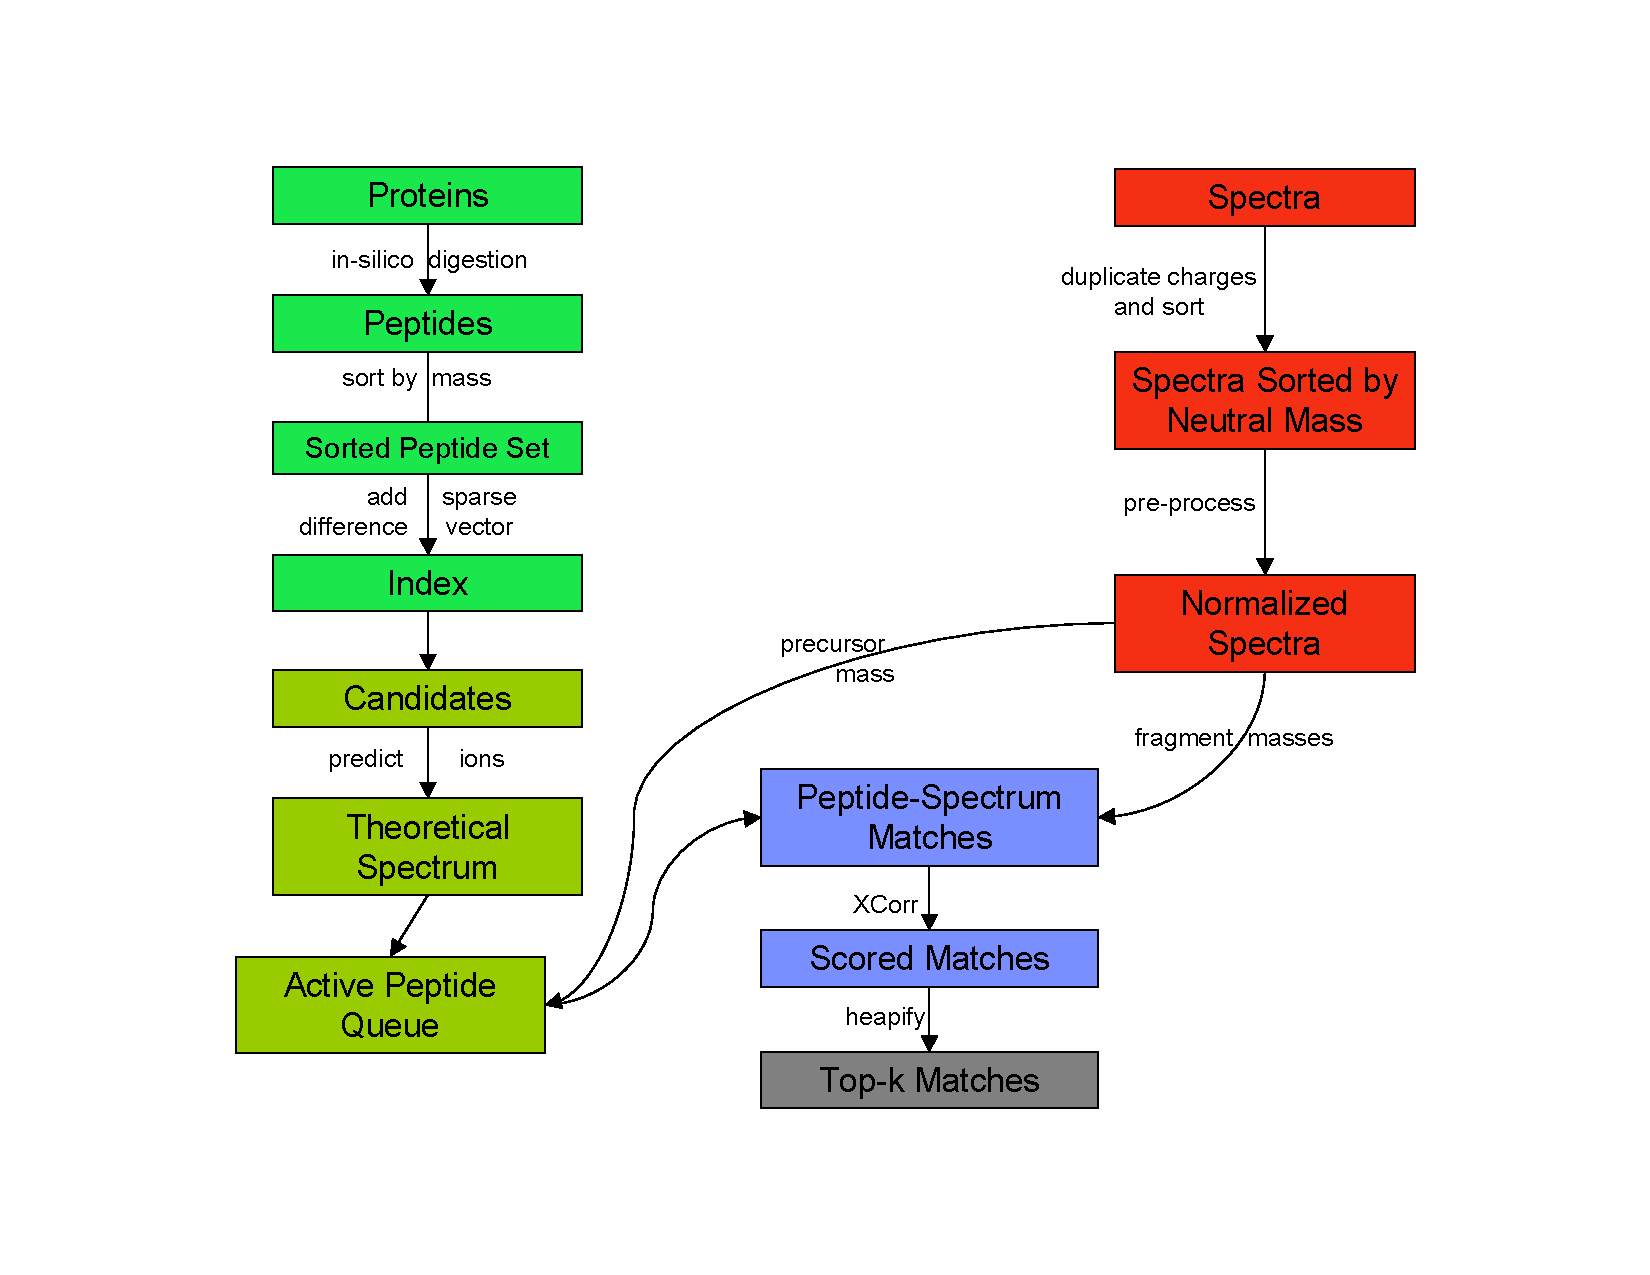
\includegraphics[width=6.0in]{Diagrams_p2-p2-cropped.pdf}
\caption{{\bf Data flow after introducing the rolling window join}
  \label{figure:join}}
\end{figure}

Crux implements an index, not present in early versions of SEQUEST,
containing all input peptides sorted by precursor mass. As each
spectrum in the input file is received, Crux seeks to the beginning of
a user defined window around the precursor mass. Then it computes the
theoretical spectrum for each peptide in that window, comparing each
successively in turn against the observed spectrum from the input. Two
significant downsides remain in this approach: there is a call to the
{\tt seek()} function 
per spectrum, and the same theoretical spectrum may be recomputed many
times over the course of a run. \tidezero did not suffer the disk seek
problem, but only because it allowed peptide sets of only very limited
size and kept them in memory.

The rolling-window join, described presently, eliminates the call to 
the {\tt seek()} function
without requiring that the whole index reside in memory, and it
eliminates significant recomputation of theoretical spectra. As
SEQUEST, Crux, and \tidezero were structured, the same theoretical
peak set is recomputed from a peptide whenever the peptide is a
candidate match for two different spectra. Rather than recompute
these, Tide creates opportunities for theoretical spectra to be reused
when possible.  To do this, Tide employs a ``rolling window'' join of
sorted peptides against sorted observed spectra.

Two changes are implemented. First, before any matching begins, all
the observed spectra are read into memory and sorted by mass.  In case
a spectrum has multiple possible charge states it appears in the
sorted array once for each charge state, as the join is performed on
the neutral (uncharged) mass.

Critics will note that reading all spectra into memory at the start is
not scalable to large sets of spectra. However, it is of much less
concern to read the spectra into memory than the candidate peptides,
since there are, for most uses, many fewer spectra than
peptides. Represented compactly, spectra can occupy about 500-1000
bytes each. Once a spectrum is evaluated, it can be discarded
completely. This suggests the following scheme as Tide scales, if
memory becomes saturated by reading in the spectra at once: at the
sorting step, one could sort spectra in batches, store to disk, and
merge the files as they were re-read as input to the join. Because Tide
is CPU-bound, disk-based costs of doing this merge could be managed by
threading. All of this is independent of the join method itself.

After the spectra are sorted, the join is performed as follows. Tide
iterates over the spectra sorted by neutral mass. At the same time,
Tide reads the presorted candidate peptides into an ``active peptide
queue.'' The queue contains just the peptides that fall within the
user-specified precursor mass window. As Tide iterates over each
successive observed spectrum, it evicts from the queue and discards
any candidate peptides whose masses are too small for the current observed
spectrum. Then Tide reads from the presorted peptide index, enqueueing
each, until it arrives at the first peptide that is too massive. This
last peptide is placed in the queue but does not fall within the
active window. The queue must support not only the standard enqueue
and dequeue operations, but also allow iteration over its contents
(without altering them). Iteration over the queue contents creates a
``rolling window,'' which occupies only as much memory as is required
to store a window's worth of theoretical spectra. This enables reuse
of the computation of the theoretical spectra so that no theoretical
spectrum need ever be computed more than once. No explicit call to the 
{\tt seek()} function
is ever performed.

At the stage it was implemented, this change cut Tide's running time
by 64\%, as shown in line 6 of Table~\ref{table:timing}. The changes
to the data flow of Tide, following the introduction of the rolling
window, are shown in Figure~\ref{figure:dataflow}(B).

\section{
  Making the Theoretical Peaks Vector Five-fold Sparser
  \label{subsubsection:fivefold}
}

Theoretical spectra in the SEQUEST algorithm occur in groups
corresponding to cleavage events, with somewhat predictable spacing
among the peaks within a group. It is possible to take advantage of
such peak groupings to represent the complete set of theoretical peaks
even more sparsely.

As explained above, the theoretical peaks vector includes ten peaks
per amino acid: the $b$-ion and $y$-ion, each with intensity 50; the
two bins flanking each of the $b$- and $y$-ions, each with intensity
25 (four peaks total); the neutral loss of ammonia for each $b$- and
$y$-ion, each with intensity 10 (two peaks); the neutral loss of water
from each $b$-ion with intensity 10; and the $a$-ion with intensity
10. The same pattern is repeated for all the ions of charge two.

Importantly, the position of some of these ions is fixed relative
to the positions of some others. This is not always true, but it is
approximately so:
\begin{enumerate}
\item The flanking ions around each of the $b$- and $y$-ions are always
  one bin away on either side.
\item The peak for the neutral loss of ammonia is usually 17 bins away
  from the corresponding $b$- and $y$-ions, but is occasionally (0.014\%
  of the time) 18 bins away. For charge-2 ions, the neutral loss of
  ammonia is either at 8 or 9 bins away, about half the time at each.
\item The peak for the neutral loss of water is usually 18 bins away
  from the corresponding $b$-ion, but is occasionally (0.0015\% of the
  time) 19 bins away. For charge-2 %b%-ions, the neutral loss of water is
  either usually at 9 bins away, but occasionally (0.46\% of the time)
  10 bins away.
\item The peak for the $a$-ion is usually 28 bins away from the
  corresponding $b$-ion, but is sometimes (0.014\% of the time) 27 bins
  away. For charge-2 ions, the corresponding $a$-ion is usually at 14
  bins away, but 8.6\% of the time is 13 bins away.
\end{enumerate}
These observations suggests the following optimization, which is implemented in
Tide. Rather than compute all ten (or 20 for charge-2) peaks for each
amino acid in each peptide, we compute only the $b$- and $y$-ion. At the
time of spectrum preprocessing, we compute a larger cache, consisting
not only of the scaled vectors Peak10, Peak25, and Peak50 but also the
following new vectors:
\begin{verbatim}
PeakY1[i] = Peak50[i] + Peak25[i-1] + Peak25[i+1] + Peak10[i-17];
PeakB1[i] = PeakY1[i] + Peak10[i-18] + Peak10[i-28];
\end{verbatim}
These vectors represent the relative positions of the peaks that get added
together as we take dot products in most cases. Similar cache vectors
are computed for the charge-2 versions in each of the two forms where
ammonia is 8 or 9 bins away.

With these cached values, a theoretical vector five times sparser than
before may be used to compute the dot product. However, some bins
will be wrong for some peptides, because the neutral-loss peaks
are not always the same distance from the $b$- and $y$-ions. Therefore,
for each theoretical spectrum we compute the very sparse vector, $s$,
of just $b$- and $y$-ions and we separately compute the original sparse
vector of peaks, $r$, which gives the correct calculations, and then
take the difference $r-s \equiv d$. Because $r$ and $s$ are often the same, $d$ is
often empty, and when not, is very sparse. By computing $s$, $r$, and $d =
r-s$, for each theoretical spectrum we can compute the dot product:
$\langle u,s \rangle + \langle u,d\rangle$ in place of $\langle u,r
\rangle$ where $u$ is the observed spectrum.

At first, applying this heuristic led to almost no observable change in performance (see line 9
of Table~\ref{table:timing}); however, the profile as shown in
Figure~\ref{figure:profiles}(c) shifted: the largest consumer of time
is no longer the dot product, but rather the computation of $d$. This
is an improvement, since the computation of $d$ has not been optimized
at this point. In fact, optimizing the computation of $d$ is not
necessary: $d$ is so sparse that it is profitable simply to
precompute it at indexing time, store it to disk and read it back
with each peptide. Line 11 of Table~\ref{table:timing} shows the 24\%
savings when $d$ gets precomputed and stored to disk.

\section{Fixed Point Arithmetic \label{subsubsection:fixedpoint}}

Another performance change breaks, albeit very slightly, the aim to
preserve exactly the output of Crux. Rather than compute the dot
product in double-precision floating-point arithmetic, Tide uses
fixed-point arithmetic. This approach is possible only because the
normalization procedure applied to the observed spectrum greatly
constrains the range of values of the intensities. To do this, Tide
multiplies each entry in the spectrum by a large constant ($10^7$) and
rounds to the nearest integer. The constraints imposed by the
normalization procedure ensure against underflow or overflow, and the
fact that the dot product is a simple summation assures numerical
stability. We therefore achieve the same results as Crux does to at
least five or six decimal places. Because of \XCorr's instability, as
mentioned above, this precision is far beyond where \XCorr values
remain meaningful. The effects of this change, however, were small on
the benchmark sets, and it remains unclear whether this change
helps. See line 12 of Table~\ref{table:timing}.

\section{FIFO Memory Allocator \label{subsubsection:fifo}}

Further profiling of a larger dataset showed that significant time
was still being spent in memory heap operations, many of which were
tied to allocating and deallocating space for theoretical spectra and
associated data.

The built-in memory allocator typical of most C and C++ programs makes
no assumptions on the order in which blocks of memory will be
allocated and deallocated. It therefore needs to keep careful track of
which blocks of memory are in use at any given time. Updating this
information as a program runs can take significant time in case many
allocation and deallocation operations are performed, as is the case
in Tide. However, in Tide, the pattern of allocations and
deallocations closely mirrors the enqueuing and dequeueing of
candidates in the active peptide queue, described in
Section~\ref{subsubsection:join}. This first-in-first-out (FIFO)
memory usage pattern is entirely predictable: if memory block $A$ is
allocated before memory block $B$, then $A$ will be freed before
$B$. This greatly simplifies the bookkeeping usually associated with
the built-in memory allocator such that the memory needed by Tide can,
for the most part, be kept in a contiguous region of machine
memory. Therefore, we introduced in Tide a specialized
first-in-first-out memory allocator that performs well on data
allocated according to the FIFO usage pattern.

\section{Compiled Dot-Product Code \label{subsubsection:compiler}}

Following the above speed improvements, profiling revealed that most
of the remaining time (about $60\%$) was spent in the dot product
computation:
\begin{verbatim}
for (int i = 0; i < num_theoretical_peaks; ++i)
  total += cache[theoretical_peaks[i]]
\end{verbatim}

This loop was already improved twice, using cache lookups instead of
multiplication operations, and using two such lookups rather than
three. Still, testing showed that unrolling this loop and hard-coding
specific values for the {\tt theoretical\_peaks} array was about twice
as fast. To illustrate the difference, suppose
{\tt theoretical\_peaks} contained these values:
{\tt 171,226,229,232,525},\ldots, etc.
Then tests showed it was roughly twice as fast as the above dot
product loop to execute:
\begin{verbatim}
total = cache[171] + cache[226] + cache[229] + cache[232] + cache[525] + ...
\end{verbatim}
The speedup is likely due to executing one less memory lookup per
array entry. But the specific values in {\tt theoretical\_peaks} are
unavailable until the theoretical peak set is computed at run
time. However, the same theoretical peak set may be reused many times.

To take advantage of this, Tide performs a run-time compilation for
each theoretical spectrum to {\tt x86} machine code to execute the
sum with preset values. The appropriate code is generated in a buffer
for each candidate peptide and the program is instructed to jump to
the buffer to run this peptide-specific dot-product code. The overall
savings is shown in line 13 of Table~\ref{table:timing}.

\bibliographystyle{unsrt}
\bibliography{refs}

\end{document}
